\documentclass[11pt,a4paper]{article}
\usepackage[T1]{fontenc}
\usepackage[utf8]{inputenc}
\usepackage[french]{babel}
\usepackage{amsmath,amssymb,booktabs,longtable,array}
\usepackage[a4paper,margin=2.25cm]{geometry}
\usepackage{graphicx}
\usepackage[hidelinks]{hyperref}
\usepackage{microtype}
\setlength{\parindent}{0pt}
\setlength{\parskip}{0.5em}

\title{Validation computationnelle du modèle M2\\
\large Corps, queue, cohortes, population et diagnostic SOC}
\author{Réplication computationnelle indépendante}
\date{3 juillet 2026}

\begin{document}
\maketitle

\begin{abstract}
Trois baselines indépendantes de 2000 pas, une grille structurelle de 36 cas et
des ablations ont été exécutées. Le verdict est mixte mais non ambigu sur les
revendications fortes. Le corps de la valeur nette n'est pas exponentiel : Fisk
gagne dans les trois seeds et l'exponentielle perd de 61 à 80 points d'AIC. Les
exposants de queue sont souvent proches de 2,8, mais une log-normale correctement
tronquée a une vraisemblance supérieure dans toutes les comparaisons ; un seed
présente en outre un saut de seuil et un exposant de 2,54 à 3,05. Les classes sont
nettement dynamiques plutôt que démographiques. Le plateau de population est
approximatif à 2000 pas, non une stationnarité établie. Enfin, une ablation longue
sans crédit reproduit queue apparente et renouvellement : l'interprétation par
auto-organisation critique du réseau de crédit n'est pas soutenue.
\end{abstract}

\tableofcontents

\section{Objectifs et protocole}

La baseline est
$(\alpha,\delta,k,\sigma,\lambda,w_0,d_0)=(1,0{,}05,6,0{,}25,10,30,28)$,
$N(0)=0$, sur 2000 pas et seeds 0, 1, 2. Un snapshot est écrit tous les 50 pas.
Les seeds et fenêtres ne sont jamais poolés entre eux.

Le corps positif est défini a priori par les quantiles 90, 95 et 97,5\,\% ; les
résultats principaux utilisent 95\,\%. Exponentielle, gamma, log-normale et Fisk
sont ajustées par maximum de vraisemblance \emph{conditionnel à la troncature
droite}. AIC et BIC utilisent respectivement un paramètre pour l'exponentielle et
deux pour les autres familles.

La queue utilise un estimateur continu de type Clauset--Shalizi--Newman : choix
de $x_{\min}$ par distance KS, puis MLE de l'exposant de densité $\alpha$. Les
fenêtres sont $[500,1000)$, $[1000,1500)$ et $[1500,2000)$. Une seconde estimation
fixe $x_{\min}$ à la médiane des trois seuils. Les intervalles sont obtenus par
100 bootstraps de blocs-snapshots. Pareto et log-normale sont comparées sur le
même domaine $x\geq x_{\min}$ ; la log-normale est normalisée par sa probabilité
de survie au seuil.

La grille de dépistage, limitée à $T=600$ et un seed, croise
$k\in\{2,3,4,6\}$, $\sigma\in\{0{,}15,0{,}25,0{,}35\}$ et
$\varepsilon_0/w_0\in\{0{,}05,0{,}25,0{,}5\}$. Elle teste la sensibilité et les
échecs démographiques, pas la stationnarité des queues. Les ablations courtes ont
le même horizon. L'ablation sans crédit est en plus prolongée à 2000 pas et
validée avec le même protocole que la baseline.

\section{Dynamique macroscopique et population}

\begin{table}[ht]
\centering
\begin{tabular}{rrrrrr}
\toprule
Seed & $N_{2000}$ & Faillites & Contrats & pente rel. $N$ & pente rel. capital \\
\midrule
0 & 1672 & 18242 & 14096 & 6,77\,\% & 13,84\,\% \\
1 & 1680 & 18379 & 13216 & 3,81\,\% & 3,25\,\% \\
2 & 1677 & 18281 & 11748 & 6,57\,\% & 2,58\,\% \\
\bottomrule
\end{tabular}
\caption{Pentes relatives extrapolées sur 1000 pas, OLS sur $[1000,2000]$.
L'autocorrélation rend les tests OLS trop optimistes ; les pentes servent de
diagnostic, pas de preuve asymptotique.}
\end{table}

\begin{figure}[ht]
\centering
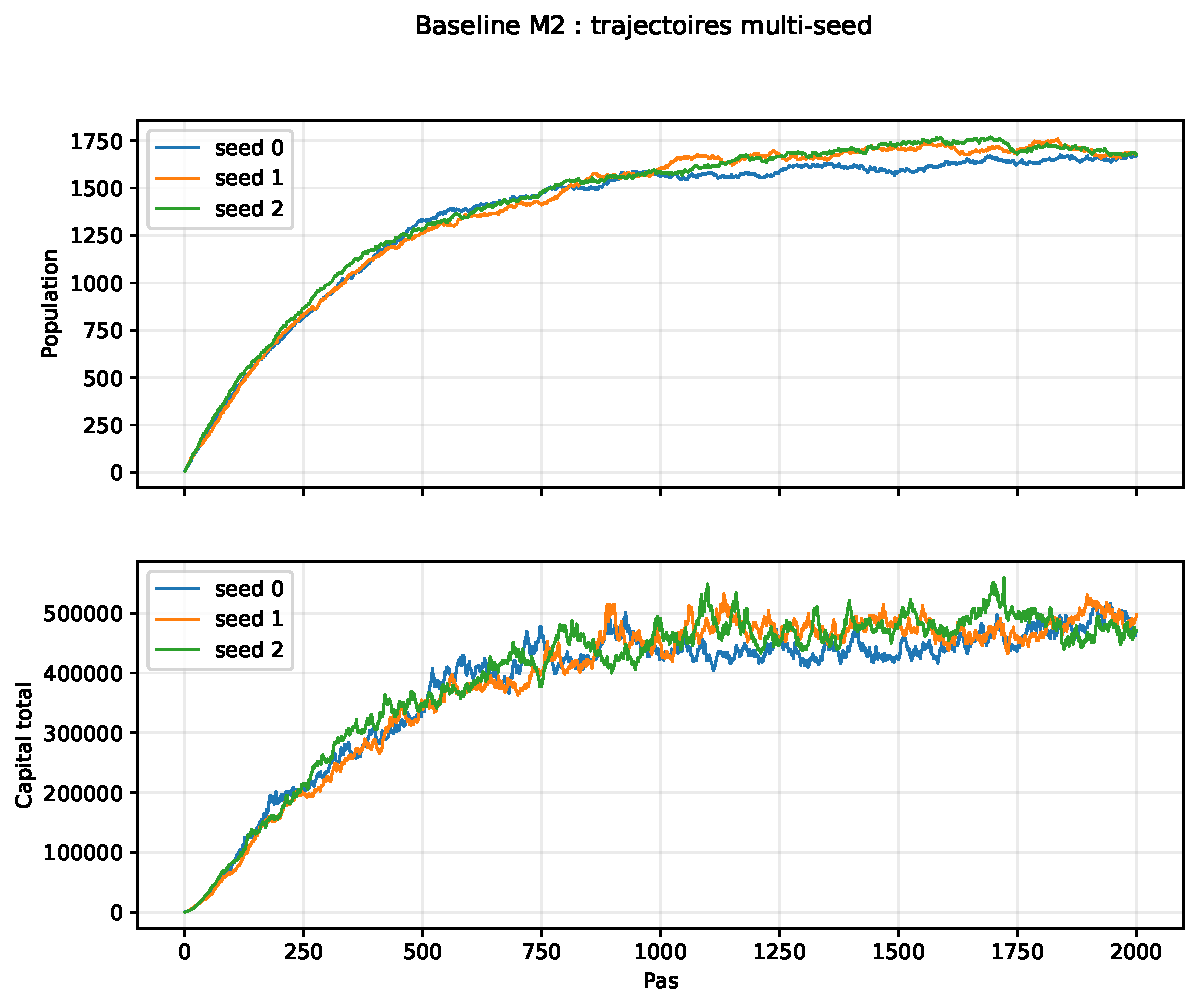
\includegraphics[width=0.95\textwidth]{figures/baseline_multiseed.pdf}
\caption{Les populations finales sont reproductibles et les trajectoires
ralentissent, mais une dérive résiduelle positive subsiste.}
\end{figure}

Le bilan naissances--décès produit donc un régime de taille finie à l'horizon
observé sans capacité exogène. Cependant, « population bornée » au sens
asymptotique n'est pas démontré : les trois pentes de population sont positives,
et le capital total dérive encore. Le résultat est classé \emph{soutien partiel},
à confirmer par des runs plus longs et une analyse de survie censurée.

La grille montre que ce bornage n'est pas robuste à la fenêtre de naissance. À
$\sigma=0{,}15$, la croissance entre $t=100$ et $t=600$ vaut 3867 à 5020 agents ;
le cas $k=2$, $\varepsilon_0/w_0=0{,}5$ ne produit aucune faillite. À
$\sigma=0{,}35$, la même croissance vaut seulement 36 à 420. Ainsi $\sigma$ et la
marge de naissance ne règlent pas seulement la forme : ils déterminent
l'existence du régime démographique sur l'horizon testé.

\begin{figure}[ht]
\centering
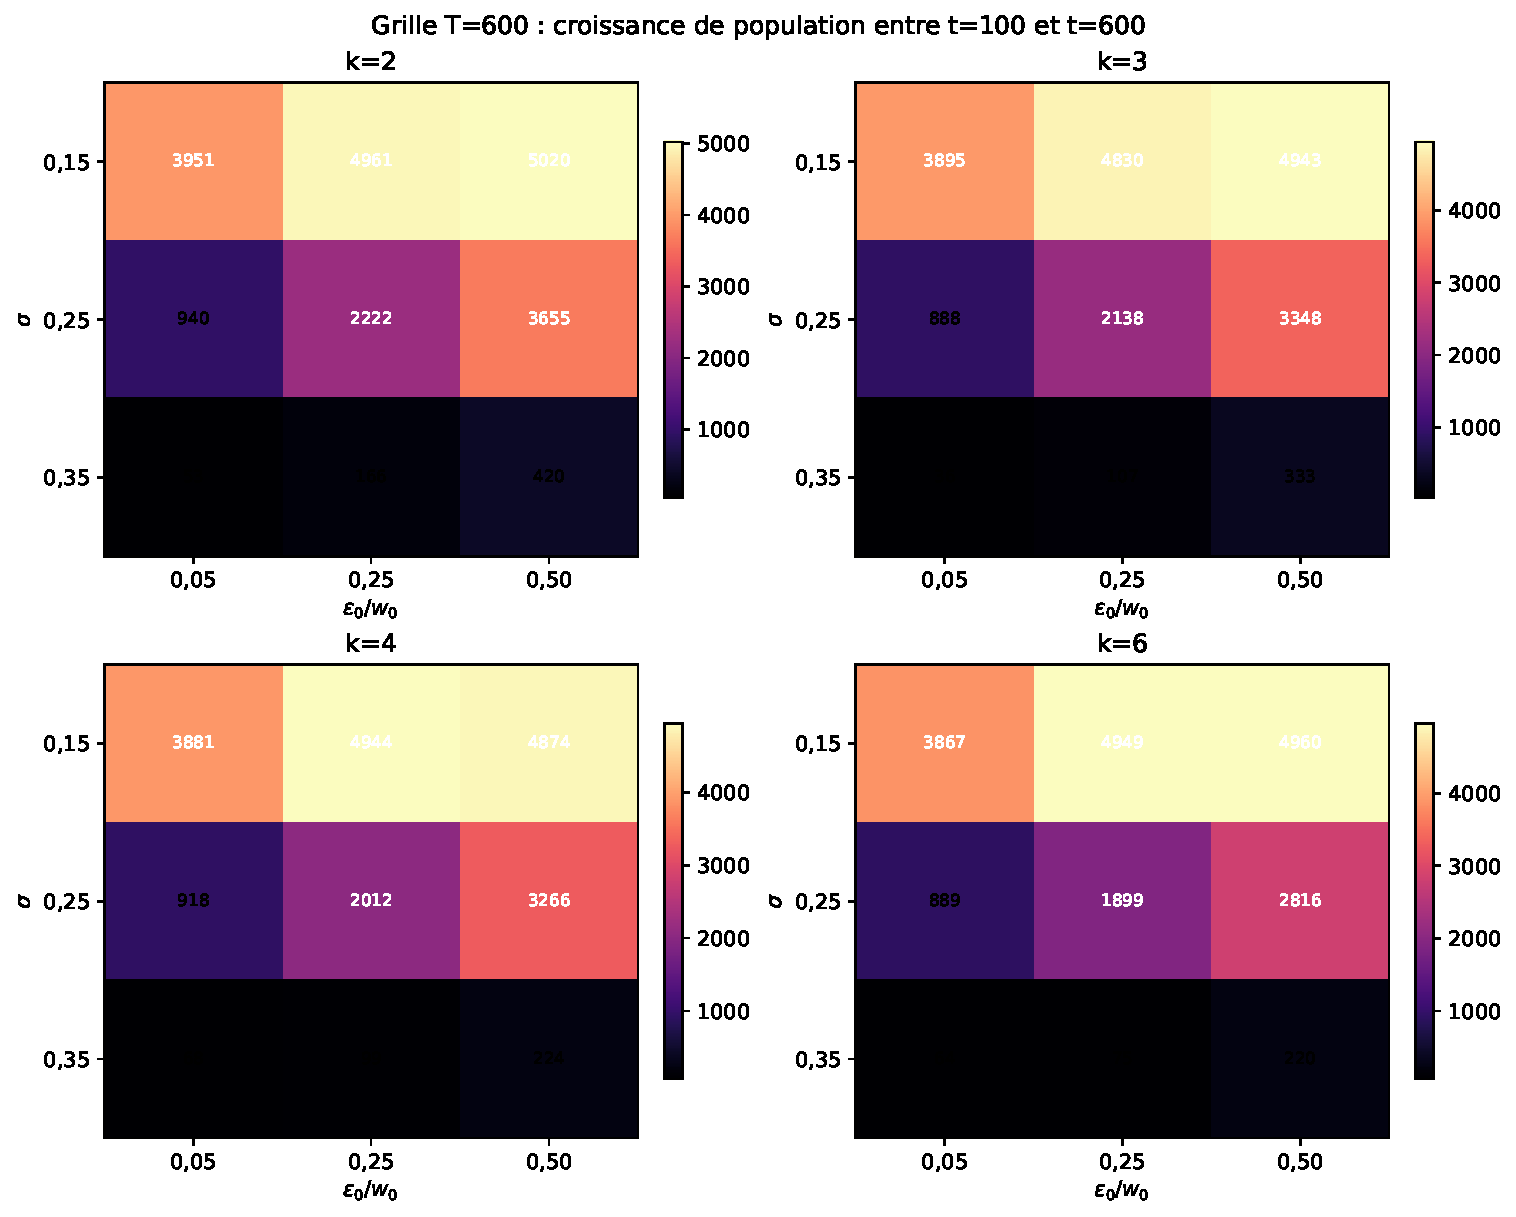
\includegraphics[width=0.9\textwidth]{figures/grid_population_growth.pdf}
\caption{Croissance de population dans la grille courte. La dépendance à
$\sigma$ et $\varepsilon_0/w_0$ est forte ; celle à $k$ est secondaire.}
\end{figure}

\section{Corps des distributions}

\begin{table}[ht]
\centering
\begin{tabular}{rrrrl}
\toprule
Seed & médiane/moyenne & meilleur modèle & $\Delta$AIC exp. & $\mathbb E[\Delta NW]$ corps \\
\midrule
0 & 0,662 & Fisk & 61,2 & 2,44 \\
1 & 0,668 & Fisk & 61,7 & 2,55 \\
2 & 0,676 & Fisk & 80,4 & 2,39 \\
\bottomrule
\end{tabular}
\caption{Corps positif de NW au quantile 95\,\%.}
\end{table}

Le ratio médiane/moyenne est proche de $\ln2=0{,}693$, mais ce diagnostic rapide
est trompeur : la vraisemblance rejette nettement l'exponentielle. Le verdict ne
change pas aux quantiles alternatifs. Dans les 36 cas de grille, Fisk gagne 35
fois et la log-normale une fois ; l'exponentielle ne gagne jamais.

\begin{figure}[ht]
\centering
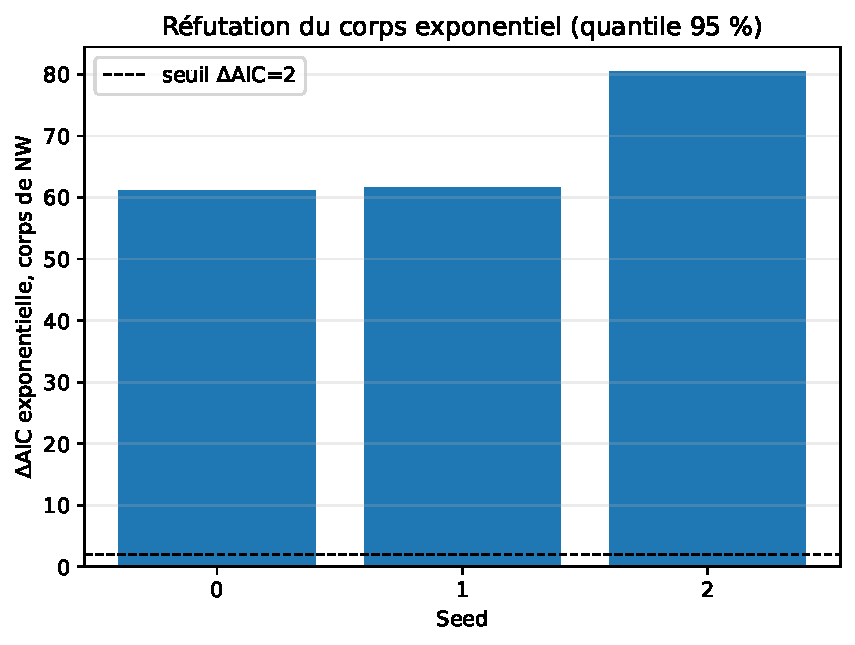
\includegraphics[width=0.68\textwidth]{figures/body_exponential_delta_aic.pdf}
\caption{L'exponentielle est très au-delà du seuil usuel $\Delta$AIC $\leq2$.}
\end{figure}

Le test mécanistique échoue également dans sa forme actuelle. Pour les agents du
corps présents au début et à la fin du pas observé, l'incrément moyen de NW est
positif (2,39 à 2,55). Avec la convention du rapport
$A_0=-\mathbb E[\Delta NW]$, on obtient $A_0<0$ et $B_0/A_0$ n'est pas une
température positive. Ce calcul est conditionné à la survie et peut être biaisé
vers le haut ; il ne suffit donc pas à réfuter toute description
Fokker--Planck, mais il ne soutient pas le mécanisme proposé.

Le capital $w$ et le revenu brut sont encore moins exponentiels sur le corps :
la log-normale gagne généralement et le ratio médiane/moyenne du revenu est
proche de 0,9. Le modèle ne produit donc pas une forme Boltzmann commune aux trois
variables.

\section{Queue : stabilité apparente, identification non acquise}

\begin{longtable}{rrrrrrr}
\toprule
Seed & fenêtre & $\alpha$ libre & $x_{\min}$ & $\alpha$ seuil fixe & LR P--LN & $p$ \\
\midrule
\endhead
0 & 500--1000 & 2,806 & 615 & 2,806 & $-0,36$ & 0,631 \\
0 & 1000--1500 & 2,845 & 648 & 2,815 & $-4,57$ & 0,080 \\
0 & 1500--2000 & 2,826 & 596 & 2,844 & $-3,31$ & 0,158 \\
1 & 500--1000 & 2,854 & 685 & 2,901 & $-3,65$ & 0,163 \\
1 & 1000--1500 & 2,874 & 748 & 2,868 & $-0,96$ & 0,455 \\
1 & 1500--2000 & 2,910 & 740 & 2,910 & $-4,01$ & 0,091 \\
2 & 500--1000 & 2,544 & 324 & 2,786 & $-25,61$ & $<10^{-3}$ \\
2 & 1000--1500 & 2,794 & 658 & 2,794 & $-0,11$ & 0,817 \\
2 & 1500--2000 & 3,054 & 857 & 2,880 & $-3,08$ & 0,225 \\
\bottomrule
\caption{Queue de NW. LR positif favoriserait Pareto ; les neuf LR sont
négatifs.}
\end{longtable}

Les seeds 0 et 1 ont des exposants libres remarquablement stables. Le seed 2
reproduit précisément le piège annoncé par le rapport : $x_{\min}$ saute de 324
à 857 et l'exposant de 2,54 à 3,05. Le seuil commun réduit cette instabilité, mais
ne résout pas l'identification de famille.

\begin{figure}[ht]
\centering
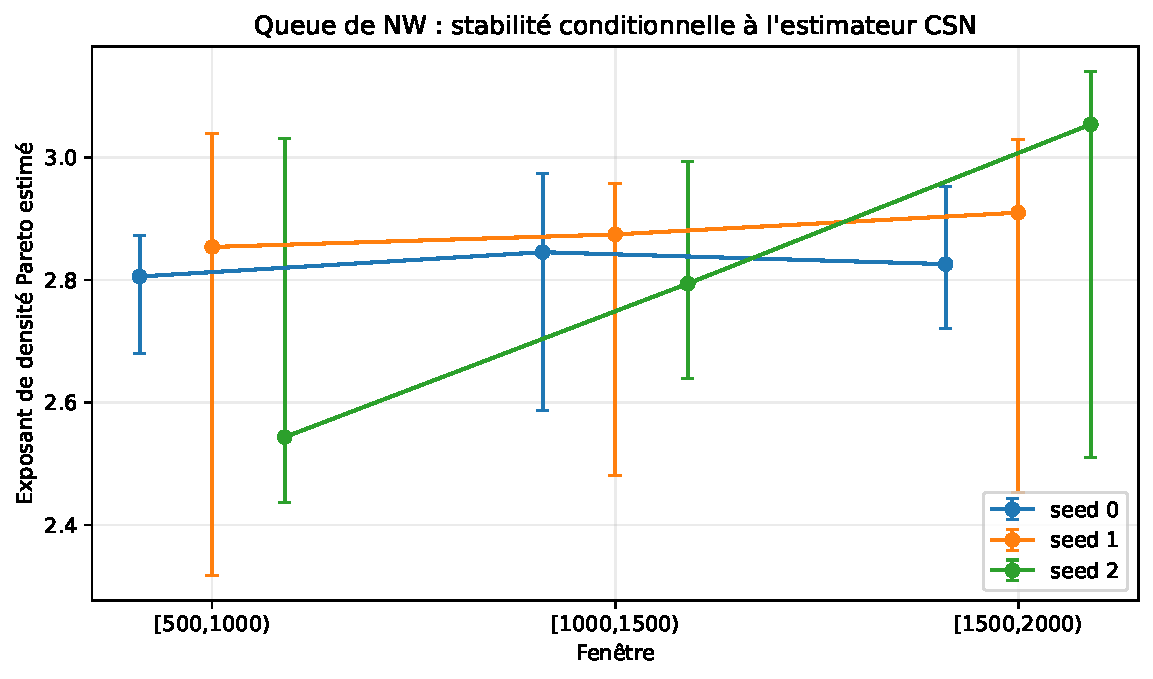
\includegraphics[width=0.88\textwidth]{figures/tail_alpha_windows.pdf}
\caption{Estimations CSN et intervalles bootstrap par blocs. Les intervalles se
recouvrent largement, mais ne constituent pas un test favorable à Pareto contre
log-normale.}
\end{figure}

La comparaison de familles est le point décisif. Les outils exploratoires du
rapport ajustaient une log-normale sur les observations de queue sans renormaliser
sa densité conditionnellement à $X\geq x_{\min}$, alors que la Pareto l'était.
Cette comparaison pénalise artificiellement la log-normale. Après correction,
tous les LR sur NW, $w$ et revenu sont négatifs. Sur NW, un seul est
significatif, mais il favorise la log-normale (seed 2, première fenêtre). Le
verdict prudent est donc : \emph{queue compatible avec une pente de type Pareto
sur une plage finie, loi de Pareto non identifiée face à la log-normale}.

Les exposants du revenu brut vont de 4,20 à 4,86, loin de ceux de NW (2,54 à
3,05). La prédiction d'un même exposant pour $y\simeq \bar r C\propto NW$ n'est
pas confirmée.

\section{Garde-fou anti-cohorte}

La corrélation Pearson âge--$\log NW$ vaut 0,155, 0,110 et 0,064 ; Spearman donne
le même ordre de grandeur. Entre $t=1000$ et $t=2000$, 86,3 à 90,6\,\% des membres
du top décile initial meurent. À $t=2000$, 90,5 à 94,6\,\% du top est né durant
les 1000 derniers pas. Le recouvrement du top initial et final est nul ou 1,2\,\%.
Les queues ajustées dans les tranches d'âge $[50,150)$ et $[150,400)$ ont des
exposants proches du transversal.

Ces résultats soutiennent fortement des classes dynamiques et réfutent une
aristocratie fondatrice immortelle. Ils n'établissent pas une structure de
classes économique : ils montrent une mobilité de rang sous forte mortalité.
La distribution d'âge reste un composant du mélange transversal, mais n'explique
pas seule la queue.

\section{SOC, cascades et ablations}

\begin{table}[ht]
\centering
\begin{tabular}{rrrrr}
\toprule
$k$ & moyenne du lot & quantile 90\,\% & maximum & $\rho$(HHI$_{t-1}$, morts$_t$) \\
\midrule
2 & 8,03 & 12 & 22 & $-0,001$ \\
3 & 7,86 & 12 & 21 & $-0,105$ \\
4 & 7,67 & 12 & 18 & $-0,233$ \\
6 & 7,85 & 11 & 19 & $-0,143$ \\
\bottomrule
\end{tabular}
\caption{Lots de faillites à $T=600$, $\sigma=0{,}25$,
$\varepsilon_0/w_0=0{,}05$. Un lot par pas mélange les déclencheurs indépendants.}
\end{table}

\begin{figure}[ht]
\centering
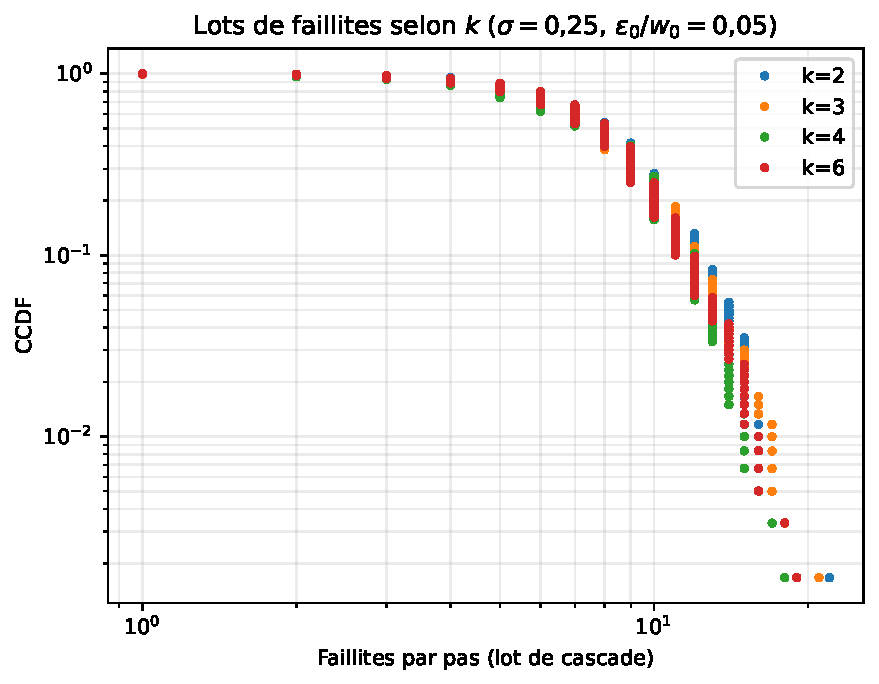
\includegraphics[width=0.7\textwidth]{figures/cascade_batches_by_k.pdf}
\caption{Aucune transition nette de taille de cascade entre $k=2$ et $k\geq3$
n'est visible sur ce diagnostic.}
\end{figure}

La plage de tailles est courte, sans preuve de loi de puissance ni de finite-size
scaling. La concentration du crédit ne prédit pas positivement les faillites du
pas suivant. Ce diagnostic est grossier, car le lot par pas n'isole pas une
avalanche ; il ne soutient néanmoins pas la boucle SOC annoncée.

L'ablation longue est plus discriminante. Sans crédit, à $T=2000$, le corps reste
Fisk ($\Delta$AIC exponentielle 85), les exposants de NW sont 2,72, 2,90 et 2,84,
la corrélation âge--$\log NW$ vaut 0,074 et la mortalité du top 85,1\,\%. Les LR
Pareto--log-normale restent négatifs. La population croît davantage
(pente relative 11,7\,\% contre 6,8\,\% pour baseline seed 0), donc le crédit
affecte le régime quantitatif, mais il n'est nécessaire ni à la queue apparente
ni au renouvellement.

\begin{figure}[ht]
\centering
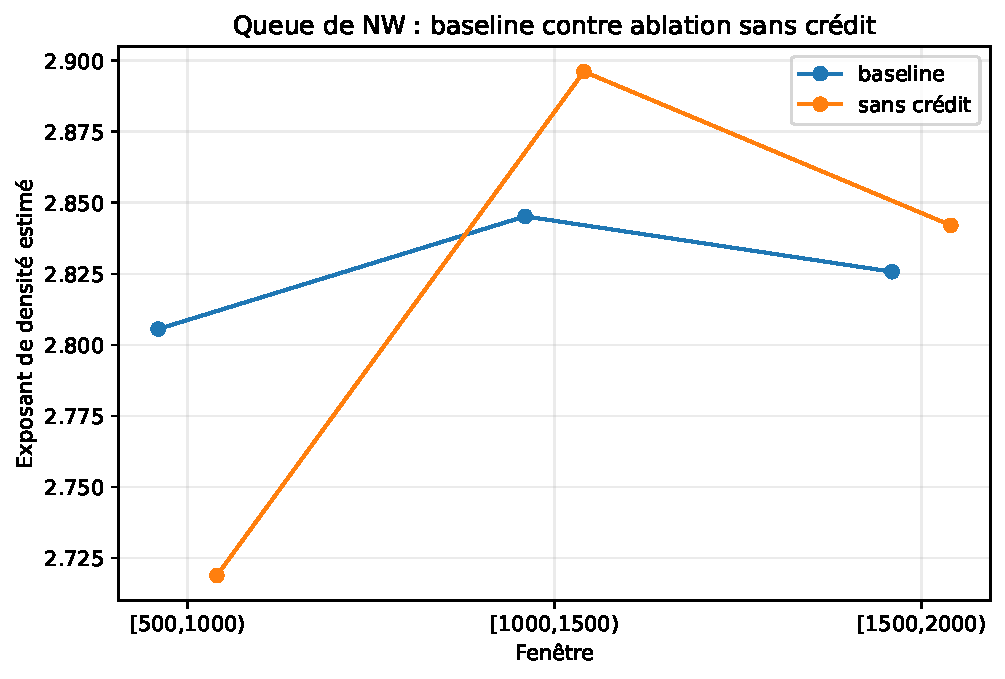
\includegraphics[width=0.72\textwidth]{figures/baseline_vs_no_credit_tail.pdf}
\caption{La suppression complète du crédit ne supprime pas les exposants de
queue observés.}
\end{figure}

À $T=600$, supprimer le choc produit zéro faillite et $N=6148$ ; supprimer le
crédit donne $N=1467$ contre 1386 pour la baseline. La source dominante de
multiplicativité, d'absorption et de renouvellement est donc le couple choc
log-normal--$d_0$, non le réseau. Le modèle peut rester intéressant comme
processus de richesse avec absorption, mais l'attribution SOC au crédit est
réfutée dans cette version.

\section{Limites}

Trois seeds ne suffisent pas à cartographier les incertitudes extrêmes. Les
fenêtres contiennent seulement dix blocs temporels, donc les bootstraps sont
larges. La grille courte ne permet pas de conclure sur les queues stationnaires.
La stationnarité est évaluée par pentes descriptives et non par test spécialisé
avec changement de régime. L'incrément du corps est conditionné à la survie. Les
lots de faillites ne sont pas des avalanches causales, ce qui limite fortement le
diagnostic SOC. Enfin, les données empiriques de richesse ou revenu ne sont pas
comparées ici : ce rapport teste les revendications internes du modèle.

\section{Prochaines expériences}

Priorités : (1) prolonger baseline et sans crédit à 4000--10000 pas ; (2) isoler
une dynamique lente de forçage et des avalanches causales ; (3) répéter les cas
frontières de la grille sur trois seeds ; (4) tester la taille via $\lambda$ et
la résolution via $(\delta/2,2T)$ ; (5) inclure les morts dans l'estimation des
incréments ; (6) comparer prédictivement Pareto, log-normale et loi de Kesten sur
des fenêtres tenues à l'écart ; (7) implémenter une liquidation simultanée.

\section{Conclusion honnête}

M2 atteint un renouvellement social net et un quasi-plateau démographique pour
la baseline. Il n'atteint pas le critère Boltzmann du corps. Sa queue a un
exposant numériquement assez stable dans deux seeds, mais n'est pas distinguée
d'une log-normale et devient instable dans le troisième. La forme n'est pas
robuste sur la grille, notamment pour la mortalité. Le crédit n'est pas nécessaire
aux signatures principales et aucun diagnostic présenté ne démontre une SOC.
Le verdict global est donc une réfutation partielle substantielle de la thèse du
rapport, avec confirmation du garde-fou anti-cohorte.

\end{document}
